%
% File naaclhlt2015.tex
%

\documentclass[11pt]{article}
\usepackage{acl2015}
\usepackage{times}
\usepackage{latexsym}
% \setlength\titlebox{5cm}    % Expanding the titlebox

%%% Custom additions %%%
% \usepackage{hyperref}
\usepackage{url}
\usepackage[leqno, fleqn]{amsmath}
\usepackage{amssymb}
\usepackage{qtree}
\usepackage{graphicx}
\usepackage{booktabs}
\usepackage{colortbl}
% \usepackage{caption}
\usepackage{subcaption}
\usepackage{xcolor}
\usepackage{color}


\newcount\colveccount
\newcommand*\colvec[1]{
        \global\colveccount#1
        \begin{bmatrix}
        \colvecnext
}
\def\colvecnext#1{
        #1
        \global\advance\colveccount-1
        \ifnum\colveccount>0
                \\
                \expandafter\colvecnext
        \else
                \end{bmatrix}
        \fi
}


\newcommand{\nateq}{\equiv}
\newcommand{\natind}{\mathbin{\#}}
%\newcommand{\natneg}{\raisebox{2px}{\tiny\thinspace$\wedge$\thinspace}}
\newcommand{\natneg}{\mathbin{^{\wedge}}}
\newcommand{\natfor}{\sqsubset}
\newcommand{\natrev}{\sqsupset}
\newcommand{\natalt}{\mathbin{|}}
\newcommand{\natcov}{\mathbin{\smallsmile}}

\newcommand{\plneg}{\mathop{\textit{not}}}
\newcommand{\pland}{\mathbin{\textit{and}}}
\newcommand{\plor}{\mathbin{\textit{or}}}

% Strikeout
\newlength{\howlong}\newcommand{\strikeout}[1]{\settowidth{\howlong}{#1}#1\unitlength0.5ex%
\begin{picture}(0,0)\put(0,1){\line(-1,0){\howlong\divide\unitlength}}\end{picture}}

\newcommand{\True}{\texttt{T}}
\newcommand{\False}{\texttt{F}}
\usepackage{stmaryrd}
\newcommand{\sem}[1]{\ensuremath{\llbracket#1\rrbracket}}

\newcommand{\mynote}[1]{{\color{blue}#1}}

\newcommand{\tbchecked}[1]{{\color{red}#1}}

\usepackage{gb4e}
\noautomath

\def\ii#1{\textit{#1}}
\newcommand{\word}[1]{\emph{#1}}

%%%%%%%%%%%%%%%%%%%%%%%%%%%%%%%%%%%%%%%%%%%%%%%%%%%%%%%%%%%%%%%%%%%%%%
%%%%% Code to simulate natbib's citealt, which prints citations with
%%%%% no parentheses:

\makeatletter
\def\citealt{\def\citename##1{{\frenchspacing##1} }\@internalcitec}
\def\@citexc[#1]#2{\if@filesw\immediate\write\@auxout{\string\citation{#2}}\fi
  \def\@citea{}\@citealt{\@for\@citeb:=#2\do
    {\@citea\def\@citea{;\penalty\@m\ }\@ifundefined
       {b@\@citeb}{{\bf ?}\@warning
       {Citation `\@citeb' on page \thepage \space undefined}}%
{\csname b@\@citeb\endcsname}}}{#1}}
\def\@internalcitec{\@ifnextchar [{\@tempswatrue\@citexc}{\@tempswafalse\@citexc[]}}
\def\@citealt#1#2{{#1\if@tempswa, #2\fi}}
\makeatother

%%%%%%%%%%%%%%%%%%%%%%%%%%%%%%%%%%%%%%%%%%%%%%%%%%%%%%%%%%%%%%%%%%%%%%


%%% %%%

\title{Recursive Neural Networks Can Learn Logical Semantics}

%\Thanks{}}

\author{
Samuel R.\ Bowman$^{\ast\dag}$ \\
\texttt{sbowman@stanford.edu} \\[2ex]
$^{\ast}$Stanford Linguistics \\
\And
Christopher Potts$^{\ast}$\\
\texttt{cgpotts@stanford.edu} \\[2ex]
$^{\dag}$Stanford NLP Group
\And
Christopher D.\ Manning$^{\ast\dag\ddag}$\\
\texttt{manning@stanford.edu}\\[2ex]
$^{\ddag}$Stanford Computer Science
}

%\author{First Author \\
%  Affiliation / Address line 1 \\
%  Affiliation / Address line 2 \\
%  Affiliation / Address line 3 \\
%  {\tt email@domain} \\\And
%  Second Author \\
%  Affiliation / Address line 1 \\
%  Affiliation / Address line 2 \\
%  Affiliation / Address line 3 \\
%  {\tt email@domain} \\}

\date{}

\makeatletter
\newcommand{\@BIBLABEL}{\@emptybiblabel}
\newcommand{\@emptybiblabel}[1]{}
\definecolor{black}{rgb}{0,0,0}
\makeatother
\usepackage[breaklinks, draft, colorlinks, linkcolor=black, urlcolor=black, citecolor=black]{hyperref}

\begin{document}
\maketitle

\begin{abstract}
Tree-structured neural networks aim to deliver a robust and principled method for representing sentence meaning, but these models largely have not outperformed simpler sequence-based models by substantial margins. We hypothesize that sequence models like LSTMs are able to discover and implicitly use the same kinds of recursive compositional structures that the tree-structured ones are built around---at least in cases where there are clear cues to that structure in the data---mitigating the advantage of the tree-structured models. We investigate this possibility by evaluating both models on an artificial task for which recursive compositional structure is crucial, and find that the sequence model is able to exploit the underlying structure, though it is less efficient at learning than the tree models, only succeeding after exposure to a larger and richer set of training data.
\end{abstract}

\section{Introduction}\label{sec:introduction}

The semantic concepts of entailment and contradiction are central to
all aspects of natural language meaning
\cite{Katz72,vanBenthem08NATLOG}, from the lexicon to the content of
entire texts. Thus, \emph{natural language
  inference} (NLI) --- characterizing and using these relations in
computational systems
\cite{dagan2006pascal,MacCartney09,maccartney2009extended} --- is
essential in tasks ranging from information retrieval to semantic
parsing to commonsense reasoning.

NLI has been addressed using a wide variety of techniques, including
those grounded in syntactic structures, knowledge bases, and symbolic
logic. In recent years, it has become an important testing ground for
approaches employing \emph{distributed} word and phrase
representations. Distributed representations excel at capturing
relations based in similarity, but it is less clear that they can be
trained to support the full range of logical inferences required for
NLI. In the SemEval 2014 task aimed at evaluating distributed
representations for NLI, the best-performing systems relied heavily on
additional features and reasoning capabilities
\cite{marelli2014semeval}.

Our primary objective in this paper is to provide a new empirical
evaluation of a wide range of models for distributed semantic
representations in the context of NLI. However, in our view, the
existing corpus resources in this area do not permit such an
assessment. They are generally too small for training modern
data-intensive, wide-coverage models, and they are often beset with
indeterminacies of event and entity coreference that significantly
impact annotation quality.

To address this, we present a new corpus of sentence pairs labeled for
entailment, contradiction, and semantic independence. At 550,152
sentence-pairs, this corpus is orders of magnitude larger than all
other resources of its type. And, in contrast to many such resources,
all of the sentences were written by humans in a grounded,
naturalistic context. In a separate validation phase, we collected
four additional judgments for each label for 56,941 of the examples,
and 98\% of cases emerge with a gold label, which attests to the high
quality of the data.

In this paper, we use this corpus to evaluate a wide variety of models
for natural language inference, including rule-based systems, simple
linear classifiers, and compositional neural networks. We find that
Tree-Structured Long Short-Term Memory networks (TreeLSTMs;
\citealt{tai2015improved,le2015compositional}) achieve the best
performance. In addition, we enhance the case for TreeLSTMs by showing
that its representations, trained on our corpus, perform well in a
disparate set of additional semantic tasks.  The success of these
transfer-learning experiments is also a testament to the centrality
of NLI in semantics.


%%%%%%%%%%%%%%%%%%%%%%%%%%%%%%%%%%%%%%%%%%%%%%%%%%%%%%%%%%%%%%%%%%%%%%


% One point of comparison that might be good to set up (maybe not in these words, this is Sam's sketch):

% Translation can also be used to train/evaluate NNs, and also demands some degree of sensitivity to compositional syntactic and semantic structure. Plus, it's easier to get good data for that task. But NLI is the better benchmark for developing NNs for language understanding, because:

% (i) Typical translation tasks require natural language generation, which is a separate difficult problem that must be learned in parallel with the semantic encoding task of interest, making results harder to interpret. We can just a vanilla well-understood classifier on top of our sentence model.

% (ii) Contradiction vs. entailment decisions in particular specifically target the abilities of NN models to learn lexical and phrasal representations (like alternation) that don't resemble similarity, either in their correlation with distributional information or their transitivity behavior. MT doesn't seem to have a good parallel to this. Since modeling similarity is almost the only aspect of NN behavior in NLP that's reasonably well understood and basically known to work, using a benchmark that explicitly demands something more sophisticated than this is likely to pay off by better exposing the weaknesses of current standard models.

% It might be also worth making an explicit comparison with sentiment as a benchmark, but that's low-hanging fruit.
\section{Testing sentence models on entailment} \label{methods}

We use the architecture depicted in Figure~\ref{fig:model:top}, which builds on the one used in \newcite{Bowman:Potts:Manning:2014}. The model architecture uses two copies of a single sentence model (a tree or sequence model) to encode the premise and hypothesis (left and right side) expressions, and then uses those encodings as the features for a multilayer classifier which predicts one of the seven relations. Since the encodings are computed separately, the sentence models must encode complete representations of the meanings of the two sentences for the downstream model to be able to succeed.

\begin{figure*}[t]
  \centering
  \begin{subfigure}[t]{0.45\textwidth}
\centering
\scalebox{0.75}{
 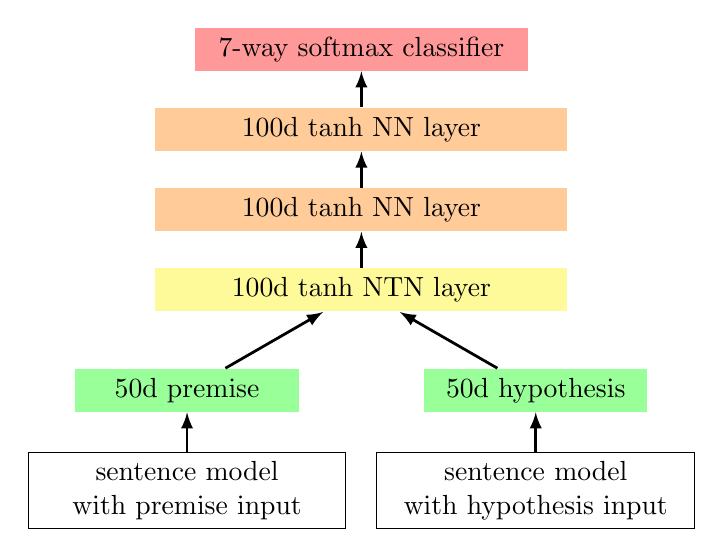
\begin{tikzpicture}
    \def\dx{21pt}
    \def\dy{29pt}

    \tikzstyle{label}=[text width=40mm,align=center]    
    \tikzstyle{softmax}=[fill=red!40,text width=40mm,align=center]
    \tikzstyle{preclass}=[fill=orange!40,text width=50mm,align=center]
    \tikzstyle{e}=[fill=green!40,text width=26mm,align=center]
    \tikzstyle{m}=[draw=black,text width=38mm,align=center]    
    
    \node[softmax]  (softmax) at (0*\dx,6*\dy) {7-way softmax classifier};
    \node[preclass]  (pc3) at (0*\dx,5*\dy) {100d $\tanh$ NN layer};
    \node[preclass]  (pc2) at (0*\dx,4*\dy) {100d $\tanh$ NN layer};
    \node[preclass,fill=yellow!40]  (pc1) at (0*\dx,3*\dy) {100d $\tanh$ NTN layer};
    \node[e]  (pe) at (-3*\dx,1.75*\dy) {50d premise};
    \node[e]  (he) at (3*\dx,1.75*\dy) {50d hypothesis};
    \node[m]  (pem) at (-3*\dx,0.5*\dy) {sentence model\\ with premise input};
    \node[m]  (hem) at (3*\dx,0.5*\dy) {sentence model\\ with hypothesis input};    
    
    \pgfsetarrowsend{latex}
    \tikzstyle{fwd} = [draw=black, line width=1pt]

          \draw [fwd] (pc3) -- (softmax);
          \draw [fwd] (pc2) -- (pc3);
          \draw [fwd] (pc1) -- (pc2);
          \draw [fwd] (pe) -- (pc1);
          \draw [fwd] (he) -- (pc1);
          \draw [fwd] (hem) -- (he);
          \draw [fwd] (pem) -- (pe);

  \end{tikzpicture}}
  
 \caption{The general architecture shared across models.}\label{fig:model:top}
  
\end{subfigure}

\begin{subfigure}[t]{0.45\textwidth}
  \centering
\scalebox{0.75}{
 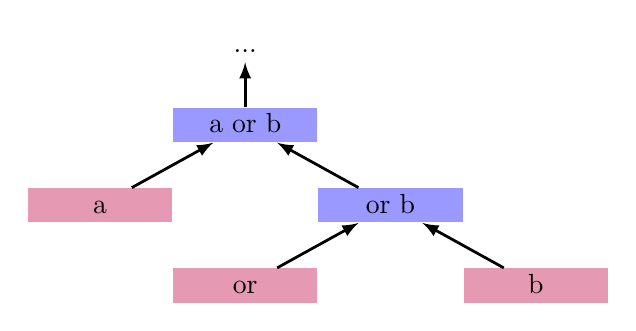
\begin{tikzpicture}
    \def\dx{21pt}
    \def\dy{29pt}


    \tikzstyle{word}=[fill=purple!40,text width=16mm,text height=2mm,align=center]
    \tikzstyle{node}=[fill=blue!40,text width=16mm,text height=2mm,align=center]
    \tikzstyle{empty}=[fill=blue!0,text width=8mm,text height=2mm,align=center]

    \node[empty]  (null) at (0*\dx,7*\dy) {...};
    \node[node]  (aorb) at (0*\dx,6*\dy) {a or b};
    \node[word]  (a) at (-2.5*\dx,5*\dy) {a};
    \node[node]  (orb) at (2.5*\dx,5*\dy) {or b};
    \node[word]  (or) at (0*\dx,4*\dy) {or};
    \node[word]  (b) at (5*\dx,4*\dy) {b};
    
    
    \pgfsetarrowsend{latex}
    \tikzstyle{fwd} = [draw=black, line width=1pt]

          \draw [fwd] (or) -- (orb);
          \draw [fwd] (b) -- (orb);
          \draw [fwd] (a) -- (aorb);
          \draw [fwd] (orb) -- (aorb);
          \draw [fwd] (aorb) -- (null);
  \end{tikzpicture}}
  
     \caption{The architecture for the TreeRNN and TreeRNTN sentence models. Terminal nodes are learned embeddings and nonterminal nodes are either NN or NTN layers with $\tanh$ nonlinearities.}\label{fig:model:tree}
  
  \end{subfigure}
 \vspace{0.5cm}
  
\begin{subfigure}[t]{0.45\textwidth}
  \centering
\scalebox{0.75}{
 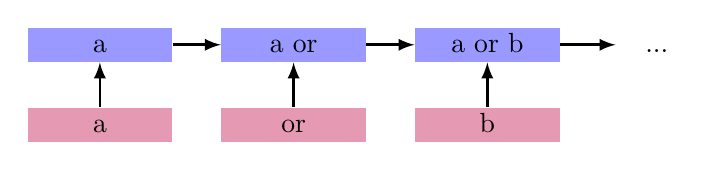
\begin{tikzpicture}
    \def\dx{35pt}
    \def\dy{29pt}


    \tikzstyle{word}=[fill=purple!40,text width=16mm,text height=2mm,align=center]
    \tikzstyle{node}=[fill=blue!40,text width=16mm,text height=2mm,align=center]
    \tikzstyle{empty}=[fill=blue!0,text width=8mm,text height=2mm,align=center]

    \node[word]  (a) at (-3*\dx,1*\dy) {a};
    \node[node]  (aN) at (-3*\dx,2*\dy) {a};
    
    \node[word]  (or) at (-1*\dx,1*\dy) {or};
    \node[node]  (orN) at (-1*\dx,2*\dy) {a or};
    
    \node[word]  (b) at (1*\dx,1*\dy) {b};
    \node[node]  (bN) at (1*\dx,2*\dy) {a or b}; 
    
    \node[empty]  (nullN) at (2.75*\dx,2*\dy) {...}; 
    
    \pgfsetarrowsend{latex}
    \tikzstyle{fwd} = [draw=black, line width=1pt]

          \draw [fwd] (or) -- (orN);
          \draw [fwd] (b) -- (bN);
          \draw [fwd] (a) -- (aN);
          \draw [fwd] (aN) -- (orN);
          \draw [fwd] (orN) -- (bN);
          \draw [fwd] (bN) -- (nullN);
          
  \end{tikzpicture}}
  
   \caption{The architecture for the LSTM sentence model. Nodes in the lower row are learned embeddings and nodes on the upper row are LSTM units.}\label{fig:model:seq}
  
    \end{subfigure}
  \caption{In our model, two copies of a sentence model---based on either tree (b) or sequence (c) models---encode the two input sentences. A multilayer classifier component (a) then uses the resulting vectors to predict a label that reflects the logical relationship between the two sentences.}
  \label{sample-figure}
\end{figure*}


\paragraph{Classifier}
The classifier component of the model consists of a combining layer which takes the two sentence representations as inputs, followed by two neural network layers, then a softmax classifier.
For the combining layer, we use a neural tensor network (NTN, \cite{chen2013learning}) layer, which sums the output of a plain recursive/recurrent neural network layer with a vector computed using two multiplications with a learned (full rank) third-order tensor parameter:
\begin{gather} 
\label{TreeRNN}
\vec{y}_{\textit{NN}} = \tanh(\mathbf{M} \colvec{2}{\vec{x}^{(l)}}{\vec{x}^{(r)}} + \vec{b}\,) \\
\label{TreeRNTN} 
\vec{y}_{\textit{NTN}} = \vec{y}_{\textit{NN}} + \tanh(\vec{x}^{(l)T} \mathbf{T}^{[1 \ldots n]} \vec{x}^{(r)})
\end{gather} 

Our model is largely identical to the model from \newcite{Bowman:Potts:Manning:2014}, but adds the two additional $\tanh$ NN layers, which we found help performance across the board, and also uses the NTN combination layer when evaluating all four models, rather than just the TreeRNTN model, so as to ensure that the sentence models are compared in as similar a setting as possible.

We only study models that encode entire sentences in fixed length vectors, and we set aside models with attention \cite{bahdanau2014neural}, a technique which gives the downstream model (here, the classifier) the potential to access each input token individually through a soft content addressing system. While attention simplifies the problem of learning complex correspondences between input and output, there is no apparent reason to believe that it should improve or harm a model's ability to track structural information like a given token's position in a tree. As such, we expect our results to reflect the same basic behaviors that would be seen in attention-based models.

\paragraph{Sentence models}
The sentence encoding component of the model transforms the (learned) embeddings of the input words for each sentence into a single vector representing that sentence. We experiment with tree-structured models (Figure~\ref{fig:model:tree}) with TreeRNN (eqn.~\ref{TreeRNN}), TreeRNTN (eqn.~\ref{TreeRNTN}), and TreeLSTM \cite{tai2015improved} activation functions. In addition, we use a sequence model (Figure~\ref{fig:model:seq}) with an LSTM activation function \cite{hochreiter1997long} implemented as in \newcite{zaremba2015recurrent}. In experiments with a simpler non-LSTM RNN sequence model, the model tended to badly underfit the training data, and those results are not included here.

\paragraph{Training} We randomly initialize all embeddings and layer parameters, and train them using minibatch stochastic gradient descent with AdaDelta \cite{zeiler2012adadelta} learning rates. Our objective is the standard negative log likelihood classification objective with L2 regularization (tuned on a separate train/test split). All models were trained for 100 epochs, after which all had largely converged without significantly declining from their peak performances.


\begin{table}[tp]
  \centering  \small
  \setlength{\arraycolsep}{8pt}
  \renewcommand{\arraystretch}{1.1}
  \newcommand{\UNK}{\cdot}  
  $\begin{array}[t]{c@{ \ }|*{7}{c}|}
    %\hline
    \multicolumn{1}{c}{}
             & \nateq     & \natfor     & \natrev     & \natneg    & \natalt     & \natcov     & \multicolumn{1}{c}{\natind} \\
    \cline{2-8}
    \nateq  & \nateq &   \natfor &  \natrev &  \natneg &   \natalt &  \natcov &  \natind \\
    \natfor & \natfor &  \natfor &  \UNK &  \natalt &   \natalt &  \UNK &  \UNK \\
    \natrev & \natrev &  \UNK &  \natrev &  \natcov &   \UNK &  \natcov &  \UNK \\
    \natneg & \natneg &  \natcov &  \natalt &  \nateq &    \natrev &  \natfor &  \natind \\
    \natalt & \natalt &  \UNK &  \natalt &  \natfor &   \UNK &  \natfor &  \UNK \\
    \natcov & \natcov &  \natcov &  \UNK &  \natrev &   \natrev &  \UNK &  \UNK \\
    \natind & \natind & \UNK &  \UNK &  \natind &  \UNK &  \UNK &  \UNK \\
    \cline{2-8}
  \end{array}$
  \caption{In \S\ref{sec:join}, we assess our models' ability to learn to do inference over pairs of relations using the rules represented here, which are derived from the definitions of the relations in Table~\ref{b-table}.  As an example, given that $p_1 \natfor p_2$ and $p_2 \natneg p_3$, the entry in the $\natfor$ row and the $\natneg$ column lets us conclude that $p_1 \natalt p_3$. Cells containing a dot correspond to situations for which no valid inference can be drawn.} 
  \label{tab:jointable}
\end{table}

\section{Reasoning about semantic relations}\label{sec:join}

The simplest kinds of deduction in natural logic involve atomic statements 
using the relations in Table~\ref{b-table}. 
For instance, from the relation $p_1 \natrev p_2$ between two propositions, 
one can infer the relation $p_2 \natfor p_1$ by applying the definitions of the relations directly. 
If one is also given the relation $p_2 \natrev p_3$ one can conclude that $p_1 \natrev p_3$, by basic set-theoretic reasoning (transitivity of $\natrev$). The
full set of sound such inferences on pairs of premise relations is depicted in
Table~\ref{tab:jointable}. Though these basic inferences do not involve compositional
sentence representations, any successful reasoning using compositional representations
will rely on the ability to perform sound inferences of this kind, so our first experiment studies how well each model can learn to perform them them in isolation.

% about the relations themselves that do not depend on the
% internal structure of the things being compared. For example, given
% that $a\sqsupset b$ and $b\sqsupset c$ one can conclude that
% $a\sqsupset c$ by the transitivity of $\sqsupset$, even without
% understanding $a$, $b$, or $c$. These seven relations support more
% than just transitivity: MacCartney and Manning's
% \cite{maccartney2009extended} join table defines 32 valid inferences
% that can be made on the basis of pairs of relations of the form $a R
% b$ and $b R' c$, including several less intuitive ones such as that if
% $a \natneg b$ and $b~|~c$ then $a \sqsupset c$.


\paragraph{Experiments}
We begin by creating a world model
on which we will base the statements in the train and test sets.
This takes the form of a small Boolean structure in which terms denote
sets of entities from a small domain.  Fig.~\ref{lattice-figure}a
depicts a structure of this form with three entities ($a$, $b$, and $c$) and eight proposition terms ($p_1$--$p_8$). We then generate a 
relational statement for each pair of terms in the model, as shown in Fig.~\ref{lattice-figure}b. 
We divide these statements evenly into train and test sets, and delete the test set
 examples which cannot be proven from the train examples, for which there is not enough information for even an ideal system to choose a correct label.
In each experimental run, we create a model with 80 terms over a domain of 7 elements, yielding a training set of 3200 examples and a test set of 
2960 examples.

We trained models with both the NN and NTN comparison functions on these
data sets.\footnote{Since this task relies crucially on the learning of a pair of vectors, no simpler version of our model is a viable baseline.} %+%
In both cases, the models are implemented as
described in \S\ref{methods}, but since the items being compared
are single terms rather than full tree structures, the composition
layer is not used, and the two models are not recursive. We simply present
the models with the (randomly initialized) embedding vectors for each
of two terms, ensuring that the model has no information about the terms
being compared except for the relations between them that appear in training.


\begin{figure}[t]
  \centering
  \begin{subfigure}[t]{0.45\textwidth}
    \centering
    \newcommand{\labelednode}[4]{\put(#1,#2){\oval(1.5,1)}\put(#1,#2){\makebox(0,0){$\begin{array}{c}#3\\\{#4\}\end{array}$}}}
    \setlength{\unitlength}{1cm}\scalebox{0.8}{
    \begin{picture}(5,5.5)
      \labelednode{2.50}{5}{}{a,b,c}
      
      \put(0.75,4){\line(3,1){1.5}}
      \put(2.5,4){\line(0,1){0.5}}
      \put(4.25,4){\line(-3,1){1.5}}
      
      \labelednode{0.75}{3.5}{p_1,p_2}{a,b}
      \labelednode{2.50}{3.5}{p_3}{a,c}
      \labelednode{4.25}{3.5}{p_4}{b,c}
      
      \put(0.75,2.5){\line(0,1){0.5}}
      \put(0.75,2.5){\line(3,1){1.5}}
      
      \put(2.5,2.5){\line(-3,1){1.5}}
      \put(2.5,2.5){\line(3,1){1.5}}
      
      \put(4.25,2.5){\line(0,1){0.5}}
      \put(4.25,2.5){\line(-3,1){1.5}}
      

      \labelednode{0.75}{2}{p_5,p_6}{a}
      \labelednode{2.50}{2}{}{b}
      \labelednode{4.25}{2}{p_7,p_8}{c}
      
      \put(2.5,1){\line(-3,1){1.5}}
      \put(2.5,1){\line(0,1){0.5}}
      \put(2.5,1){\line(3,1){1.5}}
      
      \labelednode{2.5}{0.5}{}{}
    \end{picture}}
    \caption{Example boolean structure. The terms $p_1$--$p_8$ name the sets. Not all sets have names, and  some sets have multiple names, so that learning $\nateq$ is non-trivial.}
  \end{subfigure}
  \qquad\small
    \begin{subfigure}[t]{0.43\textwidth}
    \centering \vspace{0.4cm}
    \setlength{\tabcolsep}{12pt}
    \begin{tabular}[b]{c  c}
      \toprule
      Train & Test \\
      \midrule
      $p_1 \nateq p_2$              & $p_2 \natneg p_7$ \\
      $p_1 \natrev p_5$              & $p_2 \natrev p_5$ \\
      $p_4 \natrev p_8$              & \strikeout{$p_5 \nateq p_6$} \\
      $p_5 \natalt p_7$              & \strikeout{$p_7 \natfor p_4$} \\
      $p_7 \natneg p_1$           & $p_8 \natfor p_4$ \\

      \bottomrule
    \end{tabular}

    \caption{A few examples of atomic statements about the
      model.  Test statements that are not provable from the training data shown are
      crossed out.}
  \end{subfigure}  
  \caption{Small example structure and data for learning relation composition.}
  \label{lattice-figure}
\end{figure} 

\begin{table}[tp]
  \centering\small
  \begin{tabular}{ l r@{ \ }r r@{ \ }r }
    \toprule
    ~&\multicolumn{2}{c}{Train} & \multicolumn{2}{c}{Test}\\
    \midrule
    $\natind$ only &53.8 &(10.5)    &53.8 &(10.5) \\
    15d NN &				99.8&	(99.0) &94.0&(87.0) \\
    15d NTN 				& \textbf{100} & \textbf{(100)} & \textbf{99.6} & \textbf{(95.5)}\\
    \bottomrule
  \end{tabular}
  
  
  \caption{Performance on the semantic relation experiments. These results and all other results on artificial data are reported as mean accuracy scores over five runs followed by mean macroaveraged F1 scores in parentheses. The ``$\natind$ only'' entries reflect the frequency of the most frequent class.}
  \label{joinresultstable}
\end{table}

\paragraph{Results} 
The results (Table \ref{joinresultstable}) show that NTN is able to accurately encode the relations between the terms in the geometric relations between their vectors, 
and is able to then use that information to recover relations that 
are not overtly included in the training data. The NN also generalizes fairly well, 
but makes enough errors that it remains an open question whether 
it is capable of learning representations with these properties. 
It is not possible for us to rule out the possibility that different optimization techniques or
further hyperparameter tuning could lead an NN model to succeed here.

As an example from our test data, both models correctly labeled $p_1 \natfor p_3$, potentially learning from the training examples $\{p_1 \natfor p_{51},~p_3 \natrev p_{51}\}$ or $\{p_1\natfor p_{65},~p_3 \natrev p_{65} \}$. On another example involving comparably frequent relations, the NTN correctly labeled $p_6 \natrev p_{24}$, likely on the basis of the training examples $\{p_6 \natcov p_{28},~p_{28} \natneg p_{24}\}$, while the NN incorrectly assigned it $\natind$.

% From train\test_1
\section{Recursive structure}\label{sec:recursion}

% TODO: Check on citation for clark/coecke/sadr 2011

% Run baseline anyway?

% TODO: Clean up next sent.
Recursive compositional structure is a prominent feature of natural language. 
This section examines the 
question of whether our models are able to learn a 
compositional semantics over such recursive structures.
In our evaluations, we exploit the fact that our logical language
is infinite by testing on strings that are longer and more complex
than any seen in training.

% Consider, for example, \ii{Alice said hello}, \ii{Bob said that Alice
%   said hello}, and \ii{Carl thinks that Bob said that Alice said
%   hello}. Overt recursion of this kind is easy to find, and
% theoretical accounts of natural language syntax and semantics rely
% heavily on recursive structures. In order for a model to be able to
% accurately learn natural language meanings, then, we expect that it
% would need to be able to learn to represent the meanings of function
% words in a such a way that they are able to behave correctly when
% taking their own outputs as input. In evaluating the model, we take
% advantage of the fact that recursive structures of this kind define
% potentially infinite languages by testing the model on strings that
% are longer and more complex than any seen in testing.

\paragraph{Experiments}
As in \S\ref{sec:join}, we test this phenomenon within the
framework of natural logic, but we now replace the unanalyzed symbols
from that experiment with complex formulae. These formulae
represent a truth-functionally complete classical propositional logic:
each atomic symbol is a variable over the domain \{$\True$, $\False$\}, and the only
operators are truth-functional ones.  Table~\ref{tab:pl} defines this
logic, and Table~\ref{tab:plexs} gives some examples of relational
statements that we can make in these terms. To compute these relations
between statements, we exhaustively enumerate the sets of assignments
of truth values to propositional variables that would satisfy each of
the statements, and then we convert the set-theoretic relation between
those assignments into one of the seven relations in
Table~\ref{b-table}. As a result, each relational statement represents
a valid theorem of the propositional logic.

\begin{table}[tp]
  \centering\small
  \begin{subtable}[t]{0.45\textwidth}
    \centering
    \begin{tabular}[t]{l l}
      \toprule
      Formula     & Interpretation \\
      \midrule
      $p_1$, $p_2$, $p_3$, $p_4$, $p_5$, $p_6$ & $\sem{x} \in \{\True, \False\}$ \\
      $\plneg \varphi$ & $\True$ iff $\sem{\varphi} = \False$ \\
      $(\varphi \pland \psi)$ & $\True$ iff $\False \notin \{\sem{\varphi}, \sem{\psi}\}$ \\
      $(\varphi \plor \psi)$  & $\True$ iff $\True \in \{\sem{\varphi}, \sem{\psi}\}$ \\
      \bottomrule
    \end{tabular}    
    \caption{Well-formed formulae. $\varphi$ and $\psi$
      range over all well-formed formulae, and $\sem{\cdot}$ is
      the interpretation function mapping formulae into $\{\True,
      \False\}$.}\label{tab:pl}
  \end{subtable}
  \begin{subtable}[t]{0.45\textwidth}
    \centering\vspace{4mm}
    \begin{tabular}[t]{r c l}
      \toprule
      $\plneg p_3$        & $\natneg$ & $p_3$ \\
      $\plneg \plneg p_6$ & $\nateq$  & $p_6$ \\
      $p_3$               & $\natfor$ & $(p_3 \plor p_2)$ \\
      $(p_1 \plor (p_2 \plor p_4))$               & $\natrev$ & $(p_2 \pland  \plneg p_4)$ \\
      %$(a \natfor b)$   & $\nateq$  & $(b \natrev a)$ \\	
      $\plneg\, (\plneg p_1 \pland \plneg p_2)$ & $\nateq$ & $(p_1 \plor p_2)$ \\ 
      \bottomrule
    \end{tabular}
    \caption{Examples of the type of statements used for training and testing. These are relations between
      well-formed formulae, computed in terms of sets of satisfying
      interpretation functions $\sem{\cdot}$.}\label{tab:plexs}
  \end{subtable}
  \caption{Natural logic relations over sentences of propositional logic.}  
  \label{prop-figure}
\end{table}

Socher et al.~\shortcite{socher2012semantic} show that a matrix-vector RNN
model somewhat similar to our RNTN can learn boolean logic, 
a logic where the atomic symbols are simply the
values $\True$ and $\False$. While learning the operators of that logic is not trivial, the outputs of
each operator can be represented accurately by a single bit.
In the more demanding task presented here, the atomic symbols are variables over these values, and the sentence vectors must thus be able to distinguish up to $2^{64}$ distinct conditions on valuations. Relational expressions between these conditions are essentially theorems of propositional logic, and to succeed, the model must learn to approximate the behavior of a theorem prover.
% TODO: Condense this para, and move bulk to footnote.

In our experiments, we randomly generate unique pairs 
of formulae and compute the relation that holds for each pair.
We discard pairs in which either statement is either a tautology or a
contradiction, for which the seven relations in
Table~\ref{b-table} are undefined. The resulting set of formula pairs is
then partitioned into 13 bins according the number of logical operators in
the longer of the two formulae. We then sample 20\% of each
bin for a held-out test set.

If we do not implement any constraint that the two statements being
compared are similar in any way, then the generated data are dominated
by statements in which the two formulae refer to largely separate
subsets of the six variables, which means that the $\natind$ relation
is almost always correct.  In an effort to balance the distribution of
relation labels without departing from the basic task of modeling
propositional logic, we disallow individual pairs of statements from
referring to more than four of the six propositional variables.

In order to test the model's generalization to unseen structures, we discard
training examples with more than 4 connectives, yielding 60k short training examples,
and 21k test examples containing up to 12 connectives.
We evaluated both the RNN and RNTN\footnote{We did not run any strictly simpler baselines for this experiment because it is demonstrably impossible to perform substantially above chance on longer expressions without word order information.} on the resulting data, initializing the model parameters randomly,
including the vector representations of the six variables.


\begin{figure*}[t]
  \centering
  
\includegraphics[width=5.75in]{decayfig.eps}
%  \includegraphics[width=5.3in]{recursion\string_pairwise.eps}
  \caption{Model performance on propositional logic, by expression size.}
%    The dashed line indicates that only expressions of size four or less appeared in the training data. \textbf{Bottom:} Semantically distinct formulae should have different
%    representations. As measured by Euclidean distance, only the RNTN
%    achieves this for formulae containing more than a small number of
%    connectives (\ii{and} in this example). The RNN quickly collapses the representations,
%    failing to capture the meaning contrasts.
    
  \label{prop-results} 
  
\end{figure*}


\paragraph{Results} Figure~\ref{prop-results} shows the relationship
between test accuracy and statement length. We found that both 
models were able to perform well on unseen small test examples, 
with RNN accuracy above
98\% and RNTN accuracy above 99\% on formulae below length five.
Starting at size four, performance gradually falls with increasing
size. Training accuracy was 99.4\% for the RNN and 99.8\% for the RNTN.

The performance of these models on small unseen test examples
indicates that they learned correct approximations of the underlying
logic. These approximations are accurate enough to yield
correct answers when the composition layer is only applied a small
number of times, but that the error in the approximation grows with
increasing expression size, resulting in gradually dropping performance. 
Though imperfect, model performance on the long examples is striking. 
The RNTN classifies true examples of every class but $\nateq$ 
(which occurs only once) correctly the majority of the time, where a 
typical statement might be $( ( p_1  \pland ( p_2 \plor ( \plneg p_4 ) ) ) \plor p_3 ) \natcov ( \plneg ( ( \plneg ( ( \plneg ( p_4 \plor p_3 ) )  \plor ( ( \plneg p_3 ) \plor ( \plneg p_3 ) ) ) ) \pland ( \plneg ( ( \plneg ( ( \plneg p_3 ) \plor ( \plneg p_4 ) ) ) \plor ( \plneg p_2 ) ) ) ) )$.
% TODO: Better present examples.

It appears that the RNTN model overfit somewhat relative to the plain RNN,
performing better on the training data and short examples, but worse on longer
examples. Two factors are likely involved in this: even with the lower dimension,
the RNTN composition function has about eight times as many parameters as the
RNN, and thus more capacity to find a solution involving a large number of narrow 
generalizations that work on the training data but don't generalize well. In addition,
the RNTN used here has slightly weaker L2 regularization than the 
RNN ($\lambda_{\textit{RNN}} = 0.001$, $\lambda_{\textit{RNTN}} = 0.0003$). This
yielded better average performance, but may have facilitated this effect.


% \mynote{In an effort to better understand why model performance decays, 
%we evaluated both models on pairs of long formulae involving
%binary connectives, to assess how well they distinguish representations for semantically distinct
%formulae. We found that only the RNTN is able to learn
%substantially different representations for pairs of differing formulae like $(a \pland (a \pland a))$
% and $(a \pland (a \pland b))$ when the difference between the two is placed under multiple operators.
%The RNN separates the bare symbols by a euclidean distance of 3.5, but this falls to less than one once the two are placed under three operators, and quickly approaches zero as depth increases.
% The RNTN separates the bare symbols by 2.5, and this falls off much more gradually to 1.3 with twelve operators.}

% we discovered that this model looses information about in longer
% statements in a particularly problematic way. It appears that that
% model is unable to distinguish between two sentences when the only
% difference between those sentences is embedded within a very deep
% structure. We evaluated both models on sentences that differed in only
% one term, but for which that one term was embedded under a large
% number of conjunctions, such as the pair \ii{a (and a)} and \ii{a (and
%   b)}, or the pair \ii{a (and (a (and a)))} and \ii{a (and (a (and
%   b)))}. We then measured the Euclidean distance between the vector
% representations of the two sentences in each pair. Our findings are
% shown in Figure~\ref{prop-falloff}, and show that while the RNTN can
% distinguish the two sentences well at every size that we test, the RNN
% fails after a depth of approximately six.



\section{Reasoning with quantifiers and negation}\label{sec:quantifiers}

We have seen that recursive NNs can learn an approximation of propositional
logic.  However, natural languages can express functional meanings of
considerably greater complexity than this.  As a step towards
investigating whether our models can capture this complexity, we now
directly measure the degree to which they are able to
develop suitable representations for the semantics of natural language
quantifiers like \ii{most} and \ii{all} as they interact with negation. Quantification 
and negation are far from
the only place in natural language where complex functional meanings
are found, but they are natural starting point, since they can be tested
in sentences whose structures are otherwise quite simple, and since they have
formed a standard case study in prior formal work on natural
language inference \cite{Icard:Moss:2013:LILT}.

\paragraph{Experiments}
Our experimental data consist of pairs of sentences generated from a
small artificial grammar. Each sentence contains a quantifier, a noun
which may be negated, and an intransitive verb which may be
negated. We use the basic quantifiers \ii{some}, \ii{most}, \ii{all},
\ii{two}, and \ii{three}, and their negations \ii{no}, \ii{not-all},
\ii{not-most}, \ii{less-than-two}, and \ii{less-than-three}. We also
include five nouns, four intransitive verbs, and the negation symbol
\ii{not}. In order to be able to define relations between sentences
with differing lexical items, we define the lexical relations between
each noun--noun pair, each verb--verb pair, and each
quantifier--quantifier pair. The grammar accepts aligned pairs of
sentences of this form and calculates the natural logic relationship
between them.  Some examples of these data are provided in (\ref{p1}--\ref{p3}) below.
  As in previous sections, the goal of
learning is then to assign these relational labels accurately to
unseen pairs of sentences.

%nouns = ['warthogs', 'turtles', 'mammals', 'reptiles', 'pets']
%verbs = ['walk', 'move', 'swim', 'growl']
%dets = ['all', 'not_all', 'some', 'no', 'most', 'not_most', 'two', 'lt_two', 'three', 'lt_three']
%adverbs = ['', 'not']

% To assign relation labels to sentence pairs, we built a small
% task-specific implemenation of MacCartney's logic that can
% accurately label sentences of this restricted language. The logic is
% not able to derive all intuitively true relations of this language,
% and fails to derive a single unique relation for certain types of
% statement, including De Morgean's laws (e.g. \ii{(all pets) growl
% $\natneg$ (some pet) (not growl)}), and we simply discard these
% examples. Exhaustively generating the valid sentences under this
% grammar and choosing those to which a relation label can be assigned
% yields 66k sentence pairs. Some examples of these data are provided
% in Table~\ref{examplesofdata}.

In each run, we sample 20\% of the 60k generated pairs to test on and 
train on the remainder. In this setting, each model must learn a
complete reasoning system for the limited language and logic presented
in the training data, and must be able
to recognize all of the lexical relations between the nouns, verbs,
and quantifiers and how they interact. For instance, it might see
pairs like \eqref{p1} and \eqref{p2} in training and be required to 
then label \eqref{p3}.

\vspace{-0.6cm}
\begin{gather}
  \text{(most turtle) swim} \natalt \text{(no turtle) move}\label{p1}
  \\
  \text{(all lizard) reptile} \natfor  \text{(some lizard) animal}\label{p2}
  \\
  \text{(most turtle) reptile} \natalt \text{(no turtle) animal}\label{p3}
\end{gather}\vspace{-0.8cm}

\begin{table}[tp]
  \centering \small
  \begin{tabular}{ l r@{ \ }r r@{ \ }r r@{ \ }r }
    \toprule
    ~&\multicolumn{2}{c}{$\natind$ only} & \multicolumn{2}{c}{25d RNN}  & \multicolumn{2}{c}{25d RNTN}\\
    \midrule
    Train & 35.4 &(7.5) &	\textbf{100}&		\textbf{(100)}&	99.5&	(99.3)\\	
    Test & 35.4 &(7.5) &	\textbf{99.4}&\textbf{(99.5)}& \textbf{99.4} & (99.2)\\
    \bottomrule
  \end{tabular}
  \caption{Performance on the quantifier experiments, given as \% correct and macroaveraged F1.}
  \label{qresultstable}
\end{table} 
%
% do not allow a blank line --- adds too much space
%
\paragraph{Results} The results, reported in Table~\ref{qresultstable}, show that both models are able to learn to generalize the underlying logic satisfactorily. We did not observe any consistent pattern in the few errors made by either model, and errors did not tend to be consistent across runs of the experiment, suggesting that there is no fundamental obstacle to learning a perfect model for this problem.

% TODO: Baseline
\section{The SICK textual entailment challenge}\label{sec:sick}

% TODO: Something on how we can pack enough 

The specific model architecture that we use is novel, and though the underlying tree structure approach has been validated elsewhere, our experiments so far do not guarantee that it viable model for handling inference over real
natural language data. To investigate our models' ability to handle the noisy labels and the diverse range of linguistic structures seen in typical natural language data, we use the SICK textual entailment challenge corpus \cite{marelli2014sick}. The corpus consists of about 10k natural language sentence pairs, labeled with \ii{entailment}, \ii{contradiction}, or \ii{neutral}. At only a few thousand distinct sentences (many of them variants on an even smaller set of template sentences), the corpus is not large enough to train a high quality learned model of general natural language, but it is the largest human-labeled entailment corpus that we are aware of, and our results nonetheless show that tree-structured NN models can learn to do inference in the real world.

Adapting to this task requires us to make a few additions to the techniques discussed in \S\ref{methods}. In order to better handle rare words, we initialized our word embeddings using 200 dimensional vectors trained with 
GloVe \cite{pennington2014glove} on data from Wikipedia. Since 200 dimensional vectors are too large to be practical in an TreeRNTN on a small dataset, a new embedding transformation layer is needed. Before any embedding is used as an input to a recursive layer, it is passed through an additional $\tanh$ neural network layer with the same output dimension as the recursive layer. This new layer aggregates any usable information from the embedding vectors into a more compact working representation. An identical layer is added to the SumNN between the word vectors and the comparison layer.

We also supplemented the SICK training data\footnote{We tuned the model using performance on a held out development set, but report performance here for a version of the model trained on both the training and development data and tested on the 4,928 example SICK test set. We also report training accuracy on a small sample from each data source.} with 600k examples of entailment data from the Denotation Graph project (DG, \citealt{hodoshimage}, also used by the winning SICK submission), a corpus of noisy automatically labeled entailment examples over image captions, the same genre of text from which SICK was drawn. We trained a single model on data from both sources, but used a separate set of softmax parameters for classifying into the labels from each source. We parsed the data from both sources with the Stanford PCFG Parser v.~3.3.1 \cite{klein2003accurate}. We also found that we were able to train a working model much more quickly with an additional technique: we collapse subtrees that were identical across both sentences in a pair by replacing them with a single head word. The training and test data on which we report performance are collapsed in this way, and both collapsed and uncollapsed copies of the training data are used in training. Finally, in order to improve regularization on the noisier data, we used dropout \cite{srivastava2014dropout} at the input to the comparison layer (10\%) and at the output from the embedding transform layer (25\%). 

\begin{table}[tp]
  \centering \small
    \begin{tabular}{ l@{\hspace{-0.25em}} r@{~~~~} r@{~~~~} r@{~~~~} r@{~~~~} }
    \toprule
        ~&\ii{neutral}&	 30d  & 			30d & 50d\\
    ~&only &SumNN  &TrRNN &TrRNTN\\ 
     \midrule
    DG Train	& 50.0 & 68.0 & 67.0 & \textbf{74.0} \\
    SICK Train	& 56.7 & 96.6 & 95.4 & \textbf{97.8} \\
    SICK Test	& 56.7 & 73.4 & 74.9 & \textbf{76.9} \\
    \midrule
    \textsc{Passive} (4\%)	& 0 		& 76  		& 68		&\textbf{88}\\   
    \textsc{Neg} (7\%)		& 0 		& 96	 		& \textbf{100} & \textbf{100}\\
    \textsc{Subst} (24\%)	& 28 		& \textbf{72}  		& 64 		&  \textbf{72}\\
    \textsc{MultiEd} (39\%)	&  \textbf{68} & 61  		&66 		& 64 \\
    \textsc{Diff} (26\%)		& \textbf{96} &  	68		&79		& \textbf{96}\\  
    \midrule
    \textsc{Short} (47\%) & 50.0 & 73.9 & 73.5		& \textbf{77.3} \\    
    \bottomrule
  \end{tabular}
  \caption{Classification accuracy, including a category breakdown for SICK test data. Categories are shown with their frequencies.}
  \label{sresultstable}
\end{table} 

\begin{table*}[htp]
  \centering\small
  \begin{tabular}{l@{~~~}cl}
    \toprule
  The patient is being helped by the doctor	& \ii{entailment} & The doctor is helping the patient (\textsc{Passive})\\
    A little girl is playing the violin on a beach & \ii{contradiction} &	There is no girl playing the violin on a beach (\textsc{Neg})\\
    
    The yellow dog is drinking water from a bottle& \ii{contradiction} &	The yellow dog is drinking water from a pot  (\textsc{Subst})\\
        A woman is breaking two eggs in a bowl & \ii{neutral} &A man is mixing a few ingredients in a bowl (\textsc{MultiEd})\\
        Dough is being spread by a man & \ii{neutral} & A woman is slicing meat with a knife (\textsc{Diff})\\
    \bottomrule
  \end{tabular}
  \caption{\label{examplesofsickdata}Examples of each category used in error analysis from the SICK test data. }
\end{table*}


\paragraph{Results} Despite the small amount of high quality training data available and the lack of resources for learning lexical labelships, the results (Table~\ref{sresultstable}) show that our tree-structured models perform competitively on textual entailment, beating a strong baseline. Neither model reached the performance of the winning system (84.6\%), but the TreeRNTN did exceed that of eight out of 18 submitted systems, including several which used sophisticated hand-engineered features and lexical resources specific to the version of the entailment task at hand. 

To better understand our results, we manually annotated a fraction of the SICK test set, using mutually exclusive categories for passive/active alternation pairs (\textsc{Passive}), pairs differing only by the presence of negation (\textsc{Neg}), pairs differing by a single word or phrase substitution (\textsc{Subst}), pairs differing by multiple edits (\textsc{MultiEd}), and pairs with little or no content word overlap (\textsc{Diff}). Examples of each are in Table \ref{examplesofsickdata}. We annotated 100 random examples to judge the frequency of each category, and  continued selectively annotating until each category contained at least 25. We also use the category \textsc{Short} for pairs in which neither sentence contains more than ten words.
 
The results (Table \ref{examplesofsickdata}) show that the TreeRNTN performs especially strongly in the two categories which pick out specific syntactic configurations, \textsc{Passive} and \textsc{Neg}, suggesting that that model has learned to encode the relevant structures well. It also performs fairly on \textsc{Subst}, which most closely parallels the lexical entailment inferences addressed in \S\ref{sec:quantifiers}. In addition, none of the models perform dramatically better on the \textsc{Short} pairs than on the rest of the data, suggesting that the performance decay observed in \S\ref{sec:recursion} may not impact models trained on typical natural language text.

It is known that a model can perform well on SICK (like other natural language inference corpora) without taking advantage of compositional syntactic or semantic structure \cite{marelli2014semeval}, and our summing baseline model is powerful enough to do this. Our tree models nonetheless perform substantially better, and we remain confident that given sufficient data, it should be possible for the tree models, and not the summing model, to learn a truly high-quality solution.

\section{General discussion}\label{sec:discussion}

This paper evaluated two recursive models on a series of three increasingly
challenging interpretive tasks involving natural language inference:
the core labelal algebra of natural logic with entailment and
exclusion; recursive propositional logic structures; and statements
involving quantification and negation. The results suggest that RNTNs,
but not plain RNNs, have the capacity to meet the challenges of these
tasks with reasonably-sized training sets. These positive results are
promising for the future of learned representation models in the
applied modeling of compositional semantics.

Of course, challenges remain. In terms of our experimental data, even
the RNTN falls short of perfection in our more complex tasks, with
performance falling off steadily as the depth of recursion grows. It
remains to be seen whether these deficiencies can be overcome with
improvements to the model, the optimization procedures, or the
linguistic representations
\cite{sochergrounded,kalchbrenner2014convolutional}. In addition,
there remain subtle questions about how to fairly assess whether these
models have truly generalized in the way we want them to. There is a
constant tension between showing the models training data that gives
them a chance to learn the target logical functions and revealing the
answer to them in a way that leads to overfitting. The underlying
logical theories provide only limited guidance on this point.
%
%, and the fact that there is a finite universe of possible
%  expressions makes his an unavoidable issue. 
%
%  CP: I don't understand the above. It is false if taken literally;
%  our PL generates an infinte number of formulae.
%
Finally, we have only scratched the surface of the logical complexity
of natural language; in future experiments, we hope to test sentences
with embedded quantifiers, multiple interacting quantifiers, relative
clauses, and other kinds of recursive structure. Nonetheless, the
rapid progress the field has made with these models in recent years
provides ample reason to be optimistic that they can be trained to
meet the challenges of natural language semantics.

% These experiments represent one of the first attempts to reproduce any large fragment of the behavior of a complex logic within a neural network model, and the first attempt that we are aware of to address either the encoding of lexical labels or the learning of recursive operators. This presents considerable challenges in evaluating the particular models that we choose, since we cannot rely on prior results to establish that any particular amount or type of training data is sufficient to teach any model the structure of the logic. The positive results that we have found, however, are extremely promising for the future of learned representation models in the applied modeling of meaning. We have seen that recursive neural tensor networks are able to encode lexical labels accurately and encode recursive operators. We have also seen that both RNNs and RNTNs are able to handle the meanings of quantifiers in an inference setting in at least some cases. 

% There is ample room to build on these results. In the interest of fully mirroring the capacity of existing natural logics in learned models, it would be valuable to extend these experiments to cover other ways in which meanings are encoded in natural language, including challenges such as reasoning over sentences with transitive verbs or relative clauses. In addition, it would be highly informative to compare these results on standard recursive neural networks with other proposed learned models for sentence meaning, such as dependency tree RNNs \cite{sochergrounded}, Belief Propagation RNNs (TODO: cite), or convolutional RNNs \cite{kalchbrenner2014convolutional}.



\subsubsection*{Acknowledgments}

We thank Jeffrey Pennington, Richard Socher, and audiences at CSLI, Nuance, and BayLearn, as well as Neha Nayak for developing the SICK collapsing technique.


%\section{Introduction}
%
%
%The following instructions are directed to authors of papers accepted
%for publication in the NAACL HLT 2015 proceedings.  All authors are required
%to adhere to these specifications. Authors are required to provide 
%a Portable Document Format (PDF) version of
%their papers.  The proceedings will be printed on US-Letter paper.
%Authors from countries in which access to word-processing systems is
%limited should contact the publication chairs as soon as possible.
%
%\indent\paragraph{Note} Grayscale readability of all figures and
%graphics will be enforced for all accepted papers
%(\S\ref{ssec:accessibility}).  Apart from this, the style files and
%camera-ready requirements are unchanged from last year.
%
%\section{General Instructions}
%
%Manuscripts must be in two-column format.  Exceptions to the
%two-column format include the title, as well as the 
%authors' names and complete
%addresses (only in the final version, not in the version submitted for review), 
%which must be centered at the top of the first page (see
%the guidelines in Subsection~\ref{ssec:first}), and any full-width
%figures or tables.  Type single-spaced.  Do not number the pages.
%Start all pages directly under the top margin.  See the guidelines
%later regarding formatting the first page.
%
%%% If the paper is produced by a printer, make sure that the quality
%%% of the output is dark enough to photocopy well.  It may be necessary
%%% to have your laser printer adjusted for this purpose.  Papers that are too
%%% faint to reproduce well may not be included.
%
%%% {\bf Do not print page numbers on the manuscript.}  Write them lightly
%%% on the back of each page in the upper left corner along with the
%%% (first) author's name.
%
%The maximum length of a manuscript is eight (8) pages for the main
%conference, printed single-sided, plus two (2) pages for references
%(see Section~\ref{sec:length} for additional information on the
%maximum number of pages).  Do not number the pages.
%
%The review process is double-blind, so do not include any author information (names, addresses) when submitting a paper for review.  However, you should allocate space for the names and addresses so that they will fit in the final (accepted) version.  This is best done by either providing fake or blank names and addresses (as shown in this paper).
%
%\subsection{Electronically-available resources}
%
%NAACL HLT provides this description in \LaTeX2e{} ({\tt naaclhlt2015.tex}) and PDF
%format ({\tt naaclhlt2015.pdf}), along with the \LaTeX2e{} style file used to
%format it ({\tt naaclhlt2015.sty}) and an ACL bibliography style ({\tt naaclhlt2015.bst}).
%These files are all available at
%{\tt http://naacl2015.naacl.org}.  A Microsoft Word
%template file ({\tt naaclhlt2015.dot}) is also available at the same URL. We
%strongly recommend the use of these style files, which have been
%appropriately tailored for the NAACL HLT 2015 proceedings.
%
%
%\subsection{Format of Electronic Manuscript}
%\label{sect:pdf}
%
%For the production of the electronic manuscript you must use Adobe's
%Portable Document Format (PDF). This format can be generated from
%postscript files: on Unix systems, you can use {\tt ps2pdf} for this
%purpose; under Microsoft Windows, you can use Adobe's Distiller, or
%if you have cygwin installed, you can use {\tt dvipdf} or
%{\tt ps2pdf}.  Note 
%that some word processing programs generate PDF which may not include
%all the necessary fonts (esp. tree diagrams, symbols). When you print
%or create the PDF file, there is usually an option in your printer
%setup to include none, all or just non-standard fonts.  Please make
%sure that you select the option of including ALL the fonts.  {\em
%  Before sending it, test your {\/\em PDF} by printing it from a
%  computer different from the one where it was created}. Moreover,
%some word processor may generate very large postscript/PDF files,
%where each page is rendered as an image. Such images may reproduce
%poorly.  In this case, try alternative ways to obtain the postscript
%and/or PDF.  One way on some systems is to install a driver for a
%postscript printer, send your document to the printer specifying
%``Output to a file'', then convert the file to PDF.
%
%For reasons of uniformity, Adobe's {\bf Times Roman} font should be
%used. In \LaTeX2e{} this is accomplished by putting
%
%\begin{quote}
%\begin{verbatim}
%\usepackage{times}
%\usepackage{latexsym}
%\end{verbatim}
%\end{quote}
%in the preamble.
%`
%Additionally, it is of utmost importance to specify the {\bf
%  US-Letter format} (8.5in $\times$ 11in) when formatting the paper.
%When working with {\tt dvips}, for instance, one should specify {\tt
%  -t letter}.
%
%Print-outs of the PDF file on US-Letter paper should be identical to the
%hardcopy version.  If you cannot meet the above requirements about the
%production of your electronic submission, please contact the
%publication chairs above  as soon as possible.
%
%
%\subsection{Layout}
%\label{ssec:layout}
%
%Format manuscripts two columns to a page, in the manner these
%instructions are formatted. The exact dimensions for a page on US-letter
%paper are:
%`
%\begin{itemize}
%\item Left and right margins: 1 inch
%\item Top margin: 1 inch
%\item Bottom margin: 1 inch
%\item Column width: 3.15 inches
%\item Column height: 9 inches
%\item Gap between columns: 0.2 inches
%\end{itemize}
%	
%\noindent Papers should not be submitted on any other paper size. Exceptionally,
%authors for whom it is \emph{impossible} to format on US-Letter paper,
%may format for \emph{A4} paper. In this case, they should keep the \emph{top}
%and \emph{left} margins as given above, use the same column width,
%height and gap, and modify the bottom and right margins as necessary.
%Note that the text will no longer be centered.
%
%\subsection{The First Page}
%\label{ssec:first}
%
%Center the title, author's name(s) and affiliation(s) across both
%columns (or, in the case of initial submission, space for the names). 
%Do not use footnotes for affiliations.  Do not include the
%paper ID number assigned during the submission process. 
%Use the two-column format only when you begin the abstract.
%
%{\bf Title}: Place the title centered at the top of the first page, in
%a 15 point bold font.  (For a complete guide to font sizes and styles, see Table~\ref{font-table}.)
%Long title should be typed on two lines without
%a blank line intervening. Approximately, put the title at 1in from the
%top of the page, followed by a blank line, then the author's names(s),
%and the affiliation on the following line.  Do not use only initials
%for given names (middle initials are allowed). Do not format surnames
%in all capitals (e.g., ``Bangalore,'' not ``BANGALORE'').  The affiliation should
%contain the author's complete address, and if possible an electronic
%mail address. Leave about 0.75in between the affiliation and the body
%of the first page.
%
%{\bf Abstract}: Type the abstract at the beginning of the first
%column.  The width of the abstract text should be smaller than the
%width of the columns for the text in the body of the paper by about
%0.25in on each side.  Center the word {\bf Abstract} in a 12 point
%bold font above the body of the abstract. The abstract should be a
%concise summary of the general thesis and conclusions of the paper.
%It should be no longer than 200 words.  The abstract text should be in 10 point font.
%
%{\bf Text}: Begin typing the main body of the text immediately after
%the abstract, observing the two-column format as shown in 
%the present document.  Do not include page numbers.
%
%{\bf Indent} when starting a new paragraph. For reasons of uniformity,
%use Adobe's {\bf Times Roman} fonts, with 11 points for text and 
%subsection headings, 12 points for section headings and 15 points for
%the title.  If Times Roman is unavailable, use {\bf Computer Modern
%  Roman} (\LaTeX2e{}'s default; see section \ref{sect:pdf} above).
%Note that the latter is about 10\% less dense than Adobe's Times Roman
%font.
%
%\subsection{Sections}
%
%{\bf Headings}: Type and label section and subsection headings in the
%style shown on the present document.  Use numbered sections (Arabic
%numerals) in order to facilitate cross references. Number subsections
%with the section number and the subsection number separated by a dot,
%in Arabic numerals. 
%
%{\bf Citations}: Citations within the text appear
%in parentheses as~\cite{Gusfield:97} or, if the author's name appears in
%the text itself, as Gusfield~\shortcite{Gusfield:97}. In \LaTeX2e, the former is accomplished using
%\verb|\cite| and the latter with \verb|\shortcite| or \verb|\newcite|.
%Append lowercase letters to the year in cases of ambiguities.  
%Treat double authors as in~\cite{Aho:72}, but write as 
%in~\cite{Chandra:81} when more than two authors are involved. 
%Collapse multiple citations as in~\cite{Gusfield:97,Aho:72}.
%
%\textbf{References}: Gather the full set of references together under
%the heading {\bf References}; place the section before any Appendices,
%unless they contain references. Arrange the references alphabetically
%by first author, rather than by order of occurrence in the text.
%Provide as complete a citation as possible, using a consistent format,
%such as the one for {\em Computational Linguistics\/} or the one in the 
%{\em Publication Manual of the American 
%Psychological Association\/}~\cite{APA:83}.  Use of full names for
%authors rather than initials is preferred.  A list of abbreviations
%for common computer science journals can be found in the ACM 
%{\em Computing Reviews\/}~\cite{ACM:83}.
%
%The \LaTeX{} and Bib\TeX{} style files provided roughly fit the
%American Psychological Association format, allowing regular citations, 
%short citations and multiple citations as described above.
%
%{\bf Appendices}: Appendices, if any, directly follow the text and the
%references (but see above).  Letter them in sequence and provide an
%informative title: {\bf Appendix A. Title of Appendix}.
%
%\textbf{Acknowledgment} sections should go as a last (unnumbered) section immediately
%before the references.  
%
%\subsection{Footnotes}
%
%{\bf Footnotes}: Put footnotes at the bottom of the page. They may
%be numbered or referred to by asterisks or other
%symbols.\footnote{This is how a footnote should appear.} Footnotes
%should be separated from the text by a line.\footnote{Note the
%line separating the footnotes from the text.}  Footnotes should be in 9 point font.
%
%\subsection{Graphics}
%
%{\bf Illustrations}: Place figures, tables, and photographs in the
%paper near where they are first discussed, rather than at the end, if
%possible.  Wide illustrations may run across both columns and should be placed at
%the top of a page. Color illustrations are discouraged, unless you have verified that
%they will be understandable when printed in black ink. 
%
%\begin{table}
%\begin{center}
%\begin{tabular}{|l|rl|}
%\hline \bf Type of Text & \bf Font Size & \bf Style \\ \hline
%paper title & 15 pt & bold \\
%author names & 12 pt & bold \\
%author affiliation & 12 pt & \\
%the word ``Abstract'' & 12 pt & bold \\
%section titles & 12 pt & bold \\
%document text & 11 pt  &\\
%abstract text & 10 pt & \\
%captions & 10 pt & \\
%bibliography & 10 pt & \\
%footnotes & 9 pt & \\
%\hline
%\end{tabular}
%\end{center}
%\caption{\label{font-table} Font guide. }
%\end{table}
%
%{\bf Captions}: Provide a caption for every illustration; number each one
%sequentially in the form:  ``Figure 1. Caption of the Figure.'' ``Table 1.
%Caption of the Table.''  Type the captions of the figures and 
%tables below the body, using 10 point text.  
%
%\subsection{Accessibility}
%\label{ssec:accessibility}
%
%In an effort to accommodate the color-blind (as well as those printing
%to paper), grayscale readability for all accepted papers will be
%enforced.  Color is not forbidden, but authors should ensure that
%tables and figures do not rely solely on color to convey critical
%distinctions.
%
%\section{Length of Submission}
%\label{sec:length}
%
%The NAACL HLT 2015 main conference accepts submissions of long papers
%and short papers.  The maximum length of a long paper manuscript is
%eight (8) pages of content and two (2) additional pages of references
%\emph{only} (appendices count against the eight pages, not the
%additional two pages).  The maximum length of a short paper manuscript
%is four (4) pages and two (2) additional pages of references.
%Accepted papers will be granted an additional content page. For both
%long and short papers, all illustrations, references, and appendices
%must be accommodated within these page limits, observing the
%formatting instructions given in the present document.  Papers that do
%not conform to the specified length and formatting requirements are
%subject to be rejected without review.
%
%\section{Double-blind review process}
%\label{sec:blind}
%
%As the reviewing will be blind, the paper must not include the
%authors' names and affiliations.  Furthermore, self-references that
%reveal the author's identity, e.g., ``We previously showed (Smith,
%1991) ...'' must be avoided. Instead, use citations such as ``Smith
%previously showed (Smith, 1991) ...'' Papers that do not conform to
%these requirements will be rejected without review. In addition,
%please do not post your submissions on the web until after the
%review process is complete (in special cases this is permitted: see 
%the multiple submission policy below).
%
%We will reject without review any papers that do not follow the
%official style guidelines, anonymity conditions and page limits.
%
%\section{Multiple Submission Policy}
%
%Papers that have been or will be submitted to other meetings or
%publications must indicate this at submission time. Authors of
%papers accepted for presentation at NAACL HLT 2015 must notify the
%program chairs by the camera-ready deadline as to whether the paper
%will be presented. All accepted papers must be presented at the
%conference to appear in the proceedings. We will not accept for
%publication or presentation papers that overlap significantly in
%content or results with papers that will be (or have been) published
%elsewhere.
%
%Preprint servers such as arXiv.org and ACL-related workshops that
%do not have published proceedings in the ACL Anthology are not
%considered archival for purposes of submission. Authors must state
%in the online submission form the name of the workshop or preprint
%server and title of the non-archival version.  The submitted version
%should be suitably anonymized and not contain references to the
%prior non-archival version. Reviewers will be told: ``The author(s)
%have notified us that there exists a non-archival previous version
%of this paper with significantly overlapping text. We have approved
%submission under these circumstances, but to preserve the spirit
%of blind review, the current submission does not reference the
%non-archival version.'' Reviewers are free to do what they like with
%this information.
%
%Authors submitting more than one paper to NAACL HLT must ensure
%that submissions do not overlap significantly ($>25\%$) with each other
%in content or results. Authors should not submit short and long
%versions of papers with substantial overlap in their original
%contributions.

%%%

% \section*{Acknowledgments}

% Do not number the acknowledgment section.

\bibliographystyle{acl}
\bibliography{MLSemantics} 

\end{document}
